\chapter{Schéma entités-associations}

\begin{figure}
  \centering
  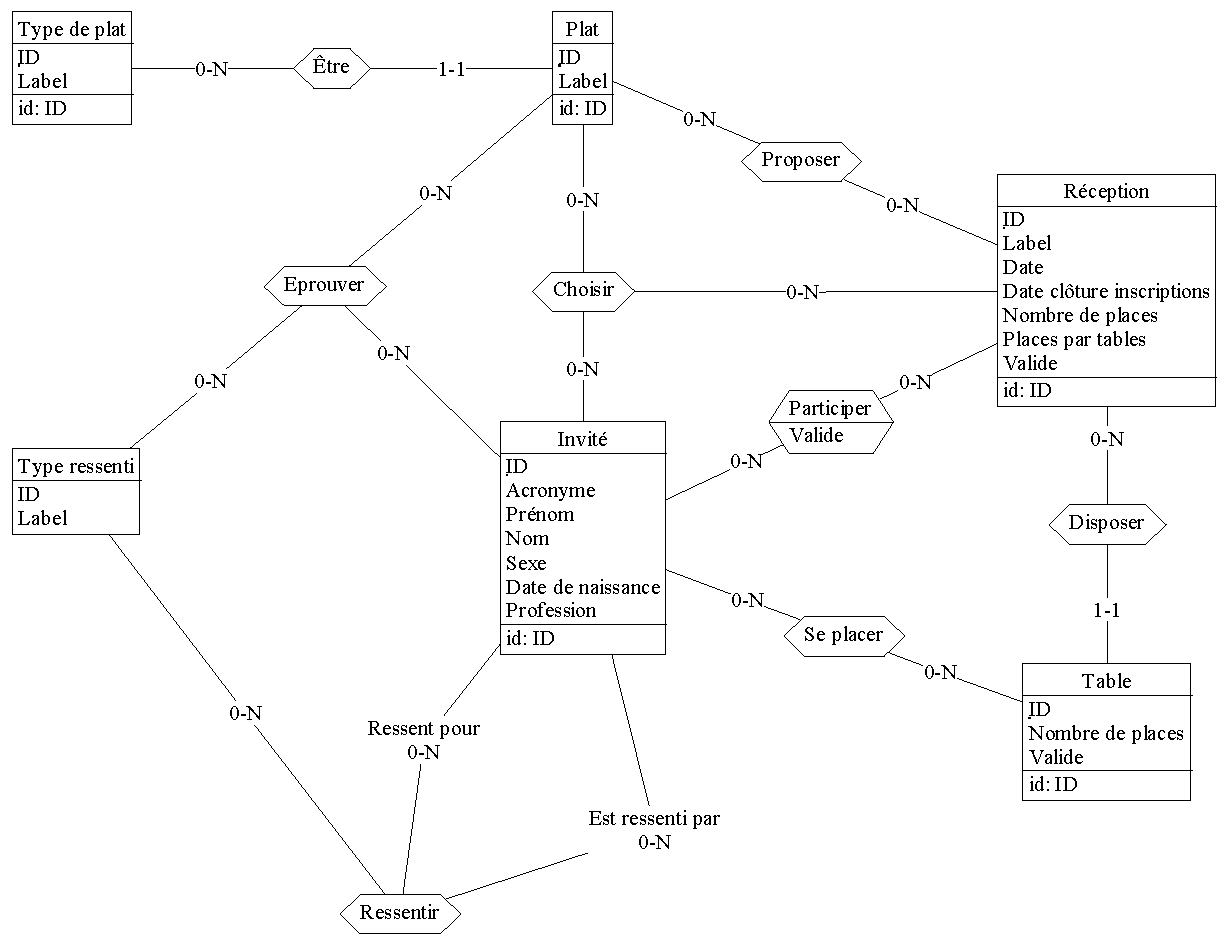
\includegraphics[angle=90]{IMG/ea}
  \caption{Schéma entités-associations}
  \label{img_ea}
\end{figure}

\begin{figure}
  \centering
  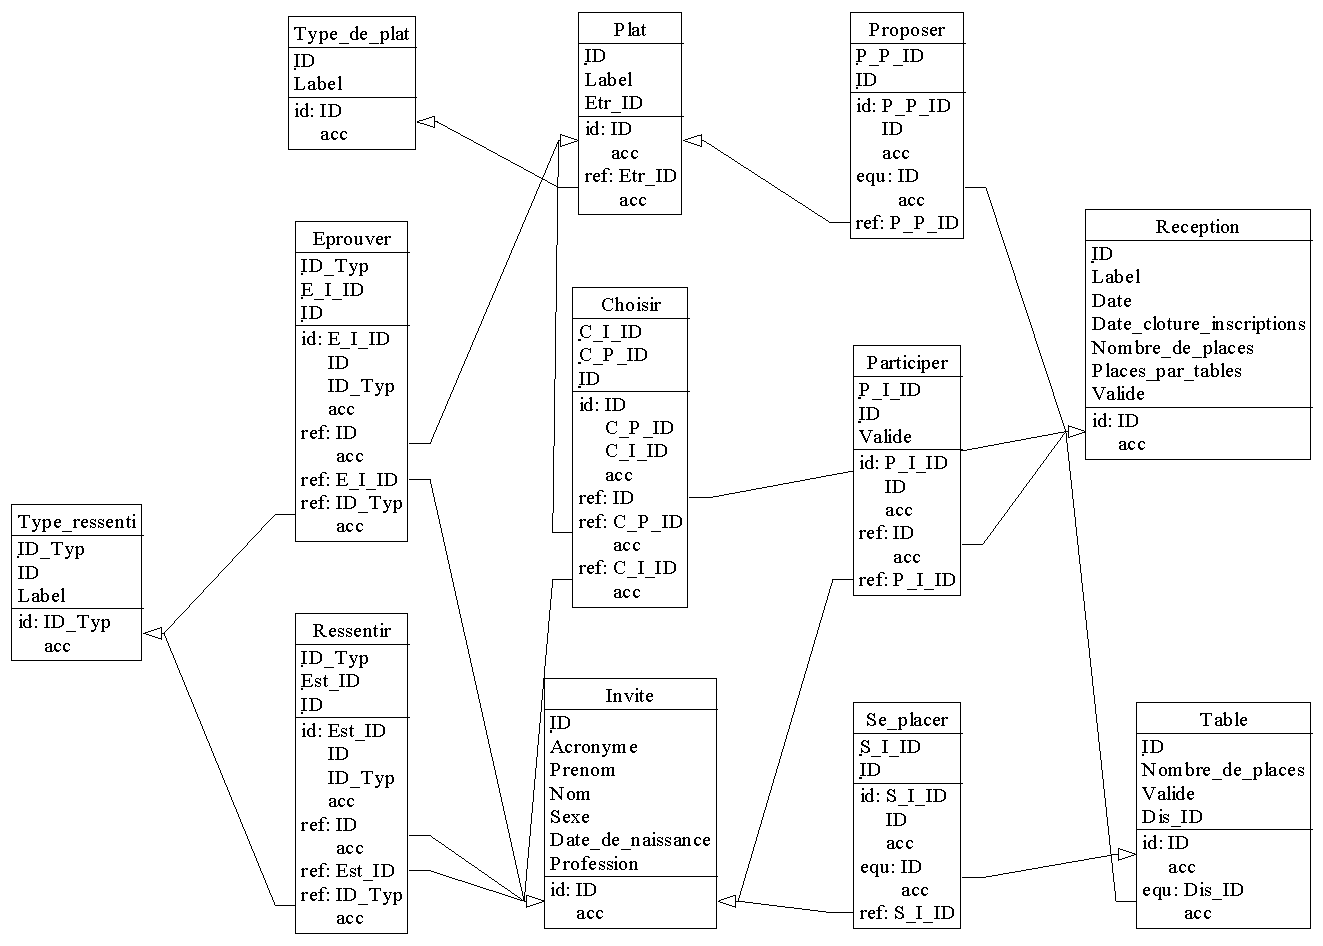
\includegraphics[angle=90]{IMG/rel}
  \caption{Schéma relationnel}
  \label{img_rel}
\end{figure}

La figure \refpage{img_ea} représente notre schéma entités-associations. Associé aux règles métier définies au chapitre \refpage{chapter_business_rules}, il permettra d'implémenter notre base de données et d'y définir nos contraintes. Le schéma relationnel résultant est illustré par la figure \refpage{img_rel}.

Ce modèle est volontairement simpliste. Il sera nécessaire de définir des vues afin de présenter au mieux les données, comme les menus ou le plan de table.